%!TEX root = ../bachelors_thesis.tex

\section{Model Overview}
For the implementation of this algorithm there was only one model that truly stood out in the sense of object orientated programming. For all other functions it proved rather difficult to find a clear class where it belonged to and also making good use of responsibilities of those classes. As mentioned in chapter \ref{chap: Background} the main work was done using syntax trees and so it was the most obvious class to build. I decided to make a extra class for the \emph{Nodes} where all the small things like setting a child, and checking if it is a root and such would be handled. \emph{Tree} and \emph{Node} could have been merge to be one class only but I found it easier to work with the code if the more standard and trivial stuff of binary trees was separated from what was more specific for this algorithm. A lot of the \emph{atomize} part is handled by the \emph{Tree} class since it works within the formula and also changes the structure of it.

The most important class however is the \emph{ProofSearch} class. It acts as a sort of main class as the initialization of the formula and the cs-list takes place here. It is also here that the methods of the \emph{Tree} class are called from. Its responsibility is to handle all algorithmic task that can be done without using a syntax tree. So the major logic of the conquer step is implemented here.

Last there is the typical \emph{Helper} class. The methods here are usually rather short  and simple and serve the purpose of making the \emph{Tree} and \emph{ProofSearch} class appear cleaner. It may be argued that some of those methods present in \emph{Helper} should be better placed in \emph{ProofSearch} and vice a verse but then again the argument for a clean object orientated model design for an algorithm is questionable and very difficult to archive.

\begin{figure}[H]
	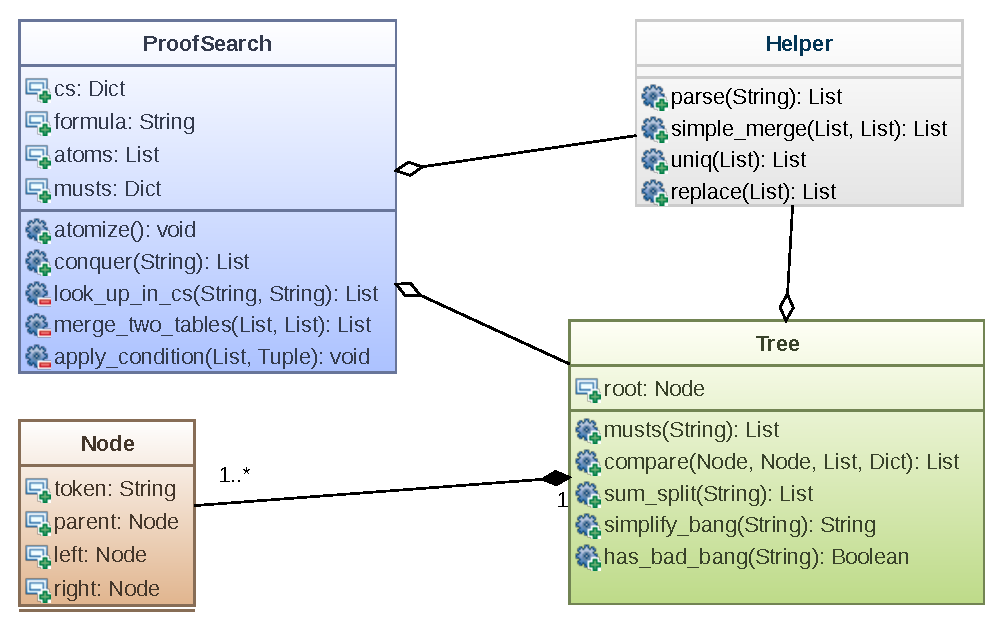
\includegraphics[width=0.9\textwidth]{/home/lyriael/BA/j-logic/thesis/Figures/uml_01.pdf}
	\caption{Simplified UML graphic of the classes used for implementing the algorithm. The list of methods and attributes is by no means complete and should simply give an idea of the construction.}
	\label{uml}
\end{figure}

\section{Important Methods}
In this section I want to show and explain some of the more complicated and important methods that make up the hear of the algorithm.

\subsection{Tree.musts}
Actually the main achievement of this method is the atomizing step, as only this simplifications made this method possible.
The algorithm takes the formula apart from top to bottom. The main cases which are differenciated are if the current operation is either a *-Operation, a !-Operation or if the term is simply a constant.

\begin{figure}[H]
    \vspace{-10pt}
	\lstinputlisting[firstline=2, lastline=22]{/home/lyriael/BA/j-logic/thesis/code_snipplets.py}
	\vspace{-10pt}
	\caption{Tree\#musts Taking a formula apart which has a * as top operation. }
	\vspace{-10pt}
\end{figure}

If for example the current justification term would be $((a*(!b)):F)$, it would be taken apart to the two subformulas $(a:(X_i\rightarrow F))$ and $((!b):(X_i))$. Because of the \emph{atomization} in the steps before it is guaranteed that every Bang is a (right) child of a Multiplication and since every Multiplication creates a new $X_i$, a term here that starts with a Bang is always on a $X_i$. Since from $!b:X_i$ follows $\exists X_j \quad s.t. \quad !b:(b:X_j)$ all $X_i$ that occurred up to now must be replaced by $(b:X_j)$. In the end we will have only proof constants remaining.

\subsection{Tree.compare}
This method is not only very tedious but gives to foundation to the method \emph{apply\_condition} which we will look at later. It basically compares each node of a tree with the corresponding of another tree. As long as the token (value) of the nodes are the same it will just process, but in case the two nodes are not identical several cases will be distinct.


\begin{figure}[H]
	\vspace{-10pt}
	\lstinputlisting[firstline=24, lastline=38]{/home/lyriael/BA/j-logic/thesis/code_snipplets.py}
	\vspace{-10pt}
\end{figure}
\begin{figure}[H]
	\vspace{-10pt}
	\lstinputlisting[firstline=41, lastline=46]{/home/lyriael/BA/j-logic/thesis/code_snipplets.py}
	\vspace{-10pt}
	\caption{Tree\#compare Here is some very verys useful text}
	\vspace{-10pt}
\end{figure}

If the current node of the term from the cs-list has a \emph{Y-wild} all other occurrences of this \emph{Y-wild} within this term will be replaces with whatever node or subtree is found in the term of the \emph{musts}. As a consequence it is possible to find a \emph{X-wild} within the term from the cs-list. Whenever that is the case, the value found in the node/subtree of the term of the \emph{musts} is a condition to this $X_i$. If the condition is merely a constant value, it will be set directly.

\subsection[ProofSearch.apply\_condition and ProofSearch.apply\_all\_conditions]{ProofSearch.apply\_condition \\and ProofSearch.apply\_all\_conditions}
\todoWriteMore{Todo}
\subsection{ProofSearch.full\_merge\_of\_two\_configs}
\todoWriteMore{Todo}

\section{Tests}
\todoWriteMore{Todo}
